\chapter{Integrals}
\thispagestyle{fancy}
Basic indefinite integrals ($c=$constant)
\begin{align}
	&\int \frac{dx}{a^2+x^2} = \frac{1}{a}\arctan\bigg(\frac{x}{a}\bigg) +c\\
	&\int \frac{dx}{\sqrt{a^2-x^2}}= \textrm{arcsin}\bigg(\frac{x}{|a|} \bigg)+c =\arctan\bigg(\frac{x}{\sqrt{a^2-x^2}} \bigg)+c\\
	&\int \frac{dx}{x+x^2} =\ln\bigg(\frac{x}{1+x} \bigg) +c\\
	&\int \frac{dx}{\sqrt{x^2-1}}= \textrm{arccosh}(x) +c\\
	&\int \frac{dx}{x\sqrt{x^2-1}}= \arccos\bigg(\frac{1}{x}\bigg)+c \\
	&\int \frac{dx}{(a^2+x^2)^{3/2}} = \frac{x}{a^2\sqrt{a^2+x^2}} +c\\
	&\int \frac{xdx}{(a^2+x^2)^{3/2}} = -\frac{1}{\sqrt{a^2+x^2}} +c\\
	&\int \frac{dx}{1-x^2} = \textrm{arctanh}(x) +c\\
	&\int \frac{dx}{\sqrt{a^2+x^2}} = \textrm{arcsinh}\bigg(\frac{x}{a}\bigg) +c = \ln\big|x+\sqrt{a^2+x^2}\big|+c\\
	&\int \frac{xdx}{1+x^2} =\frac{1}{2}\ln(1+x^2) +c\\
	&\int \frac{xdx}{\sqrt{1+x^2}}= \sqrt{1+x^2} +c\\
	&\int \frac{\sqrt{x}dx}{\sqrt{1-x}}= \arcsin(\sqrt{x})-\sqrt{x(1-x)} +c\\
	&\int \frac{x^2}{a^2+x^2} dx=\frac{-x}{2}\sqrt{a^2-x^2}+\frac{a^2}{2}\sin^{-1}\left(\frac{x}{a}\right)+c\\
	&\int \frac{1}{(a^2+x^2)^2}dx = \frac{x}{2a^2(x^2+a^2)}+\frac{1}{2a^3}\arctan\left(\frac{x}{a}\right) +c \\
	&\int \frac{x^2}{(a^2+x^2)^2}dx = \frac{-x}{2(x^2+a^2)}+\frac{1}{2a}\arctan\left(\frac{x}{a}\right) +c \\
	&\int \ln(x)=x\ln(x)-x+c 
\end{align}

\invisiblesection{Brief Table of Integrals}
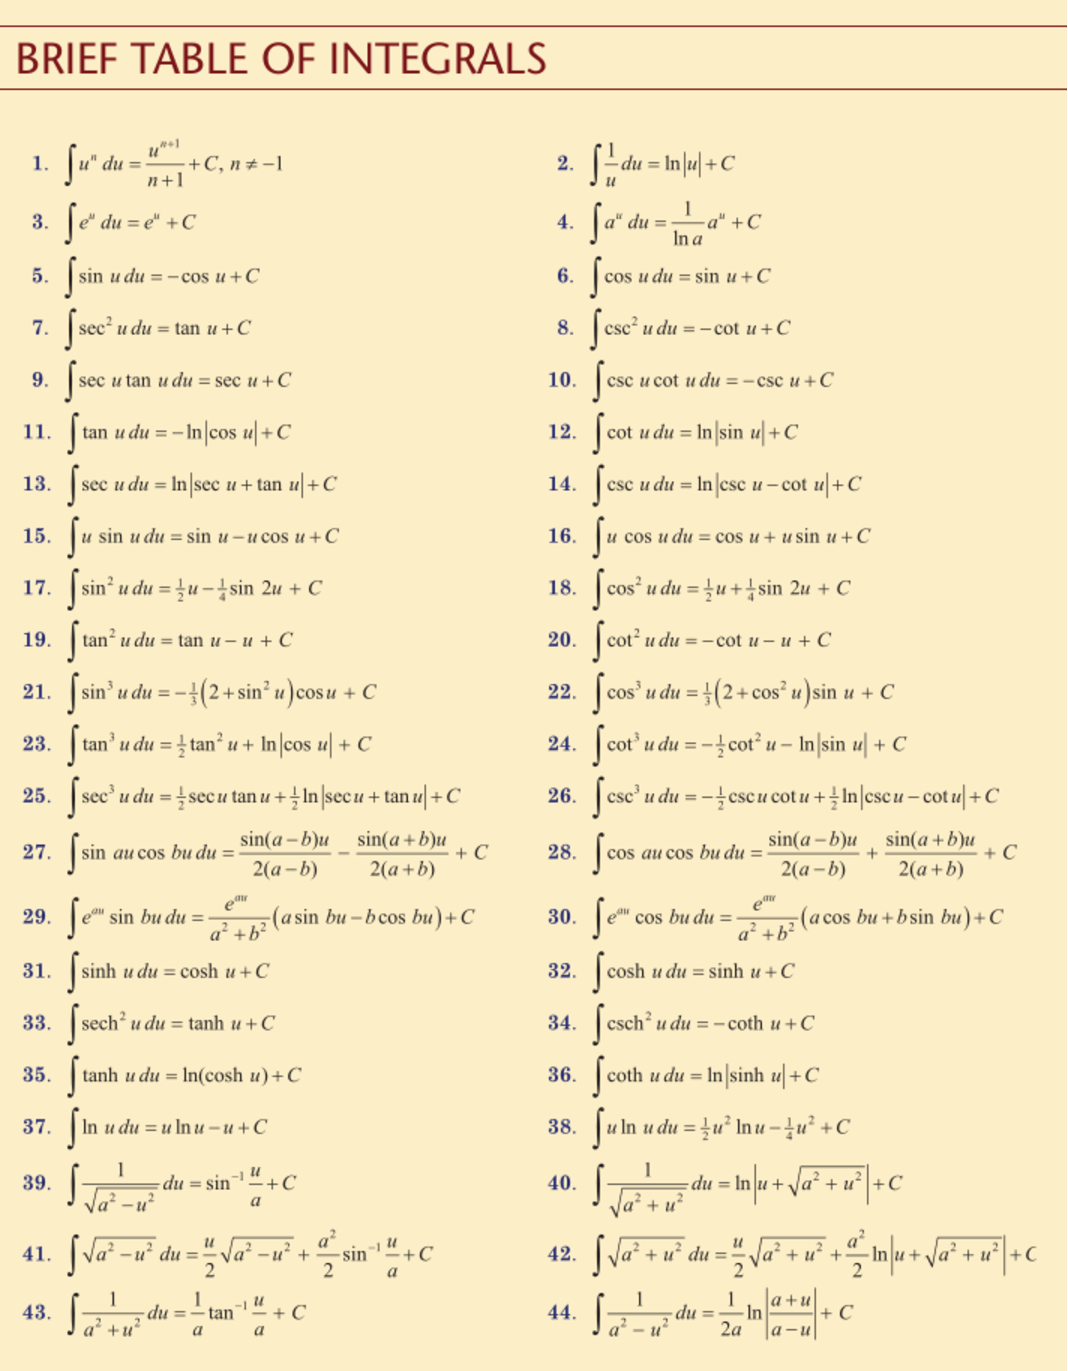
\includepdf[pages=1,pagecommand=\thispagestyle{fancy}, scale=0.8, pagecommand={\footnotetext{This "Brief Table of Integrals" is taken directly from Dennis G. Zill - A First Course in Differential Equations, 10th Ed. When time permits it will be re-created in an original format.}}]{Resources/IntegralTable}
\newpage

Exponential integrals
\begin{align}
	&\int_{-\infty}^{\infty} \frac{e^{-iax}}{(1+x^2)}dx = \pi e^{-|a|}
\end{align}
Trigonometric integrals 
\begin{align}
	&\int \tan(x)dx = -\ln(\cos(x)) +c\\
	&\int \tanh(x)dx = \ln(\cosh(x))+c \\
	&\int \sin^2(x)dx = \frac{1}{2}\big(x-\sin(x)\cos(x)\big)+c = \frac{1}{4}\big(2x-\sin(2x)\big)+c\\
	&\int \cos^2(x)dx = \frac{1}{2}\big(x+\sin(x)\cos(x)\big)+c = \frac{1}{4}\big(2x+\sin(2x)\big)+c \\
	&\int \sin^2(x)\cos(x)dx = \frac{1}{3}\sin^3(x)+c \\
	&\int \cos^2(x)\sin(x)dx = -\frac{1}{3}\cos^3(x)+c \\
	&\int \sin^3(x)dx = -\frac{1}{3}\cos(x)\big(\sin^2(x)+2\big)+c \\
	&\int x\sin^2(x)dx = \frac{1}{4}\big(x^2-x\sin(2x)-\frac{1}{2}\cos(2x)\big)+c\\
	&\int x^2\sin^2(x)dx =\frac{x^3}{6}-\bigg(\frac{x^2}{4}-\frac{1}{8}\bigg)\sin(2x)-\frac{x}{4}\cos(2x)+c \\
	&\int x^n \sin(ax)dx = -\frac{x^n}{a}\cos(ax)+ \frac{n}{a}\int x^{n-1}\cos(ax)dx \\
	&\int x^n \cos(ax)dx = \frac{x^n}{a}\sin(ax)- \frac{n}{a}\int x^{n-1}\sin(ax)dx		
\end{align}
The Wallis Cosine Formula
\begin{align}
\int_{0}^{\pi/2}\cos^n(x) dx = \int_{0}^{\pi/2}\sin^n(x) dx = \frac{(n-1)!!}{n!!}
\begin{cases}
\pi/2 &\textrm{ for } n=2,4,\dots\\
1 &\textrm{ for } n=3,5,\dots\\
\end{cases}
\end{align}




\newpage
\section{Gaussian Integrals}
The integral of an arbitrary Gaussian function is
\begin{align}
\int x^ne^{\beta x} dx = e^{\beta x}\sum_{k=0}^{n}(-1)^k\frac{n!x^{n-k}}{(n-k)!\beta^{k+1}}+c
\end{align}
Some general Gaussian integrals evaluate as
\begin{align}
\int_{-\infty}^{\infty} e^{-\alpha x^2} dx = \sqrt{\frac{\pi}{\alpha}} 
\end{align}
\begin{multicols}{2}
	\noindent
\begin{align}
I_n&=\int x^ne^{-x/\alpha}dx \\
I_0&= -\alpha e^{-x/\alpha} \\
I_1&= -(\alpha^2+\alpha x) e^{-x/\alpha} \\
I_2&= -(2\alpha^3+2\alpha^2 x+\alpha x^2) e^{-x/\alpha} \\
I_{n+1}&=\alpha^2\frac{\partial  I_n}{\partial \alpha} 
\end{align}
\begin{align}
&\int_{0}^{\infty}e^{-x/\alpha}dx = \alpha \\
&\int_{0}^{\infty}xe^{-x/\alpha}dx = \alpha^2 \\
&\int_{0}^{\infty}x^2e^{-x/\alpha}dx = 2\alpha^3 \\
&\int_{0}^{\infty}x^ne^{-x/\alpha}dx = n!\alpha^{n+1}
\end{align}
\end{multicols}
The integral of an arbitrary Gaussian function with an n-dimensional linear term (with $n \in \mathbb{Z}$) is
\begin{align}
\int_{0}^{\infty}x^{2n}e^{-\alpha x^2}dx = \sqrt{\frac{\pi}{\alpha}}\frac{(2n-1)!!}{2^{n+1}\alpha^n} &\implies  \int_{-\infty}^{\infty}x^{2n}e^{-\alpha x^2}dx = \sqrt{\frac{\pi}{\alpha}}\frac{(2n-1)!!}{(2\alpha)^n}\\
\int_{0}^{\infty}x^{2n+1}e^{-\alpha x^2}dx = \frac{n!}{2a^{n+1}} &\implies \int_{-\infty}^{\infty}x^{2n+1}e^{-\alpha x^2}dx = 0
\end{align}
Therefore a general solution is
\begin{align}
\int_{0}^{\infty}x^ne^{-\alpha x^2}dx = 
\begin{cases}
\displaystyle
\frac{(n-1)!!}{2^{n/2+1}a^{n/2}}\sqrt{\frac{\pi}{\alpha}} & \textrm{ for $n$ even} \\
\displaystyle
\frac{[\frac{1}{2}(n-1)]!}{2a^{(n+1)/2}}& \textrm{ for $n$ odd} 
\end{cases}
\end{align}
The below form of a gaussian integral evaluates to zero when $n$ is odd due to the function being odd, but when $n$ is even, the more general integral has the following closed form
\begin{align}
\int_{-\infty}^{\infty} x^ne^{-\alpha x^2+\beta x}=\sqrt{\frac{\pi}{\alpha}}e^{\beta^2/(4\alpha)}\sum_{k=0}^{\lfloor n/2\rfloor} {{n}\choose{2k}} (2k-1)!!(2a)^{k-n}\beta^{n-2k}
\end{align}
